\chapter{Architectural design}

\section{Overview}

In the S\&C application, five high-level components can be distinguished: the web server, the application server, the DBMS, the email service, and the browser interface.

The web server main objective is to deliver web pages upon user requests.
The application server is the main component of the system, as it contains every piece of business logic required to satisfy the goals specified in the RASD document.
The role of the DBMS is the usual, which is providing interaction with a database by executing command operations.
The email service is used to validate the user account at sign up time, since the verification link is sent via email.
Lastly, the browser interface is the application, in the form of web pages, that is reachable by the user from a browser.

\section{Components view}

\begin{enumerate}[label=\textbf{C\arabic* -}]

\item \htitle{Browser interface}
This is the the web application used by the client, which is reachable by any browser.
The full range of operations that it provides can only be used after the authentication process, performed by the authentication service, results successful.
It allows both students and companies to perform a certain set of actions based on the type of user.

\item \htitle{Web server}
This is the intermediary between the frontend and the backend.
Its purpose is to manage the browser UI pages independently and transparently from the point of view of the other servers components.
The web server main tasks are the static resources delivery and the web pages content retrieval and forwarding.
After receiving an HTTP request, the web server retrieves from the application server the data needed to fill the corresponding HTML template, which are then both returned to the user, along with the static style assets.

\item \htitle{DMBS}
The DBMS, which manages the DB containing all the data that the platform utilizes, stays on a separate machine.
It is then the query service component that, by providing the necessary SQL queries to other components, allows the application server to reach for the stored data.

\item \htitle{Email server}
The email server represents the external machines that the email service reaches in order to send messages.
Those machines are property of the actual email providers, but they show how the application server email service component can utilize them via their APIs.

\item \htitle{Request dispatcher}
The web server processes incoming HTTP requests by calling the appropriate application server component.
The components are responsible for retrieving the necessary data that the web server uses to populate the HTML template, which is then returned to the user.
Since different web pages may require data from different components, the request dispatcher ensures that each request is routed to the correct application server component.

\item \htitle{Authentication service}
This component provides the set of procedures required to handle the authentication of a user into the system.
It manages the log in and sign up phases.

\item \htitle{Email service}
The main goal of this component is to implement all the procedures that the server requires in order to send email messages to the user.
Mainly, this component allows the authentication service to send a verification email when handling the sign up of a user.

\item \htitle{Notification service}
The purpose of this component is to collect and manage all the notifications that a user receives.
It defines the notification types and allows other components to easily send them.

\item \htitle{Query service}
This service acts as a mediator between the server components and the DBMS.
It uses the DBMS APIs to implement a set of functions which have the sole purpose of manipulating the database or retrieving information from it.

\item \htitle{Recommendation service}
This service provides the algorithms necessary for finding suitable advertisements and candidates.
These are called when the user opens the feed in the home page, or when looking for strong matches that are to be notified.

\item \htitle{Suggestion service}
This service provides the algorithms necessary for evaluating the user profiles, in order to propose enhancements.
These are called by the profile manager component when the user provides new profile information.

\item \htitle{Profile manager}
Users must be able to insert and edit their profile information.
Validity checks and DB updates are performed by this component.
The query service and the suggestion service APIs are used when data is to be updated.

\item \htitle{Enrollment manager}
This component manages all the selection process phases, from the student application request to the start of the internship.
It also handles the questionnaires that companies send to students to fill in.

\item \htitle{Internship manager}
This component handles the operations that the internship may allow or require when it is in the ongoing status.
Along initializing and interrupting the internship, it permits users to visualize its annex information.

\item \htitle{Complaint manager}
This component allows students and companies to send complaints regarding an ongoing internship, hence allowing the university to visualize and handle them.
Since complaints must have a valid reference to an ongoing internship, the internship manager component APIs are here used.

\item \htitle{Feedback manager}
When an internship ends, both parties are requested to fill in a feedback form.
This component handles this operation, by sending, receiving and acting accordingly to the feedback forms content.
Since feedback forms must have a valid reference to an internship that has concluded, the internship manager component APIs are here used.

\end{enumerate}

\begin{figure}[H]
    \centering
    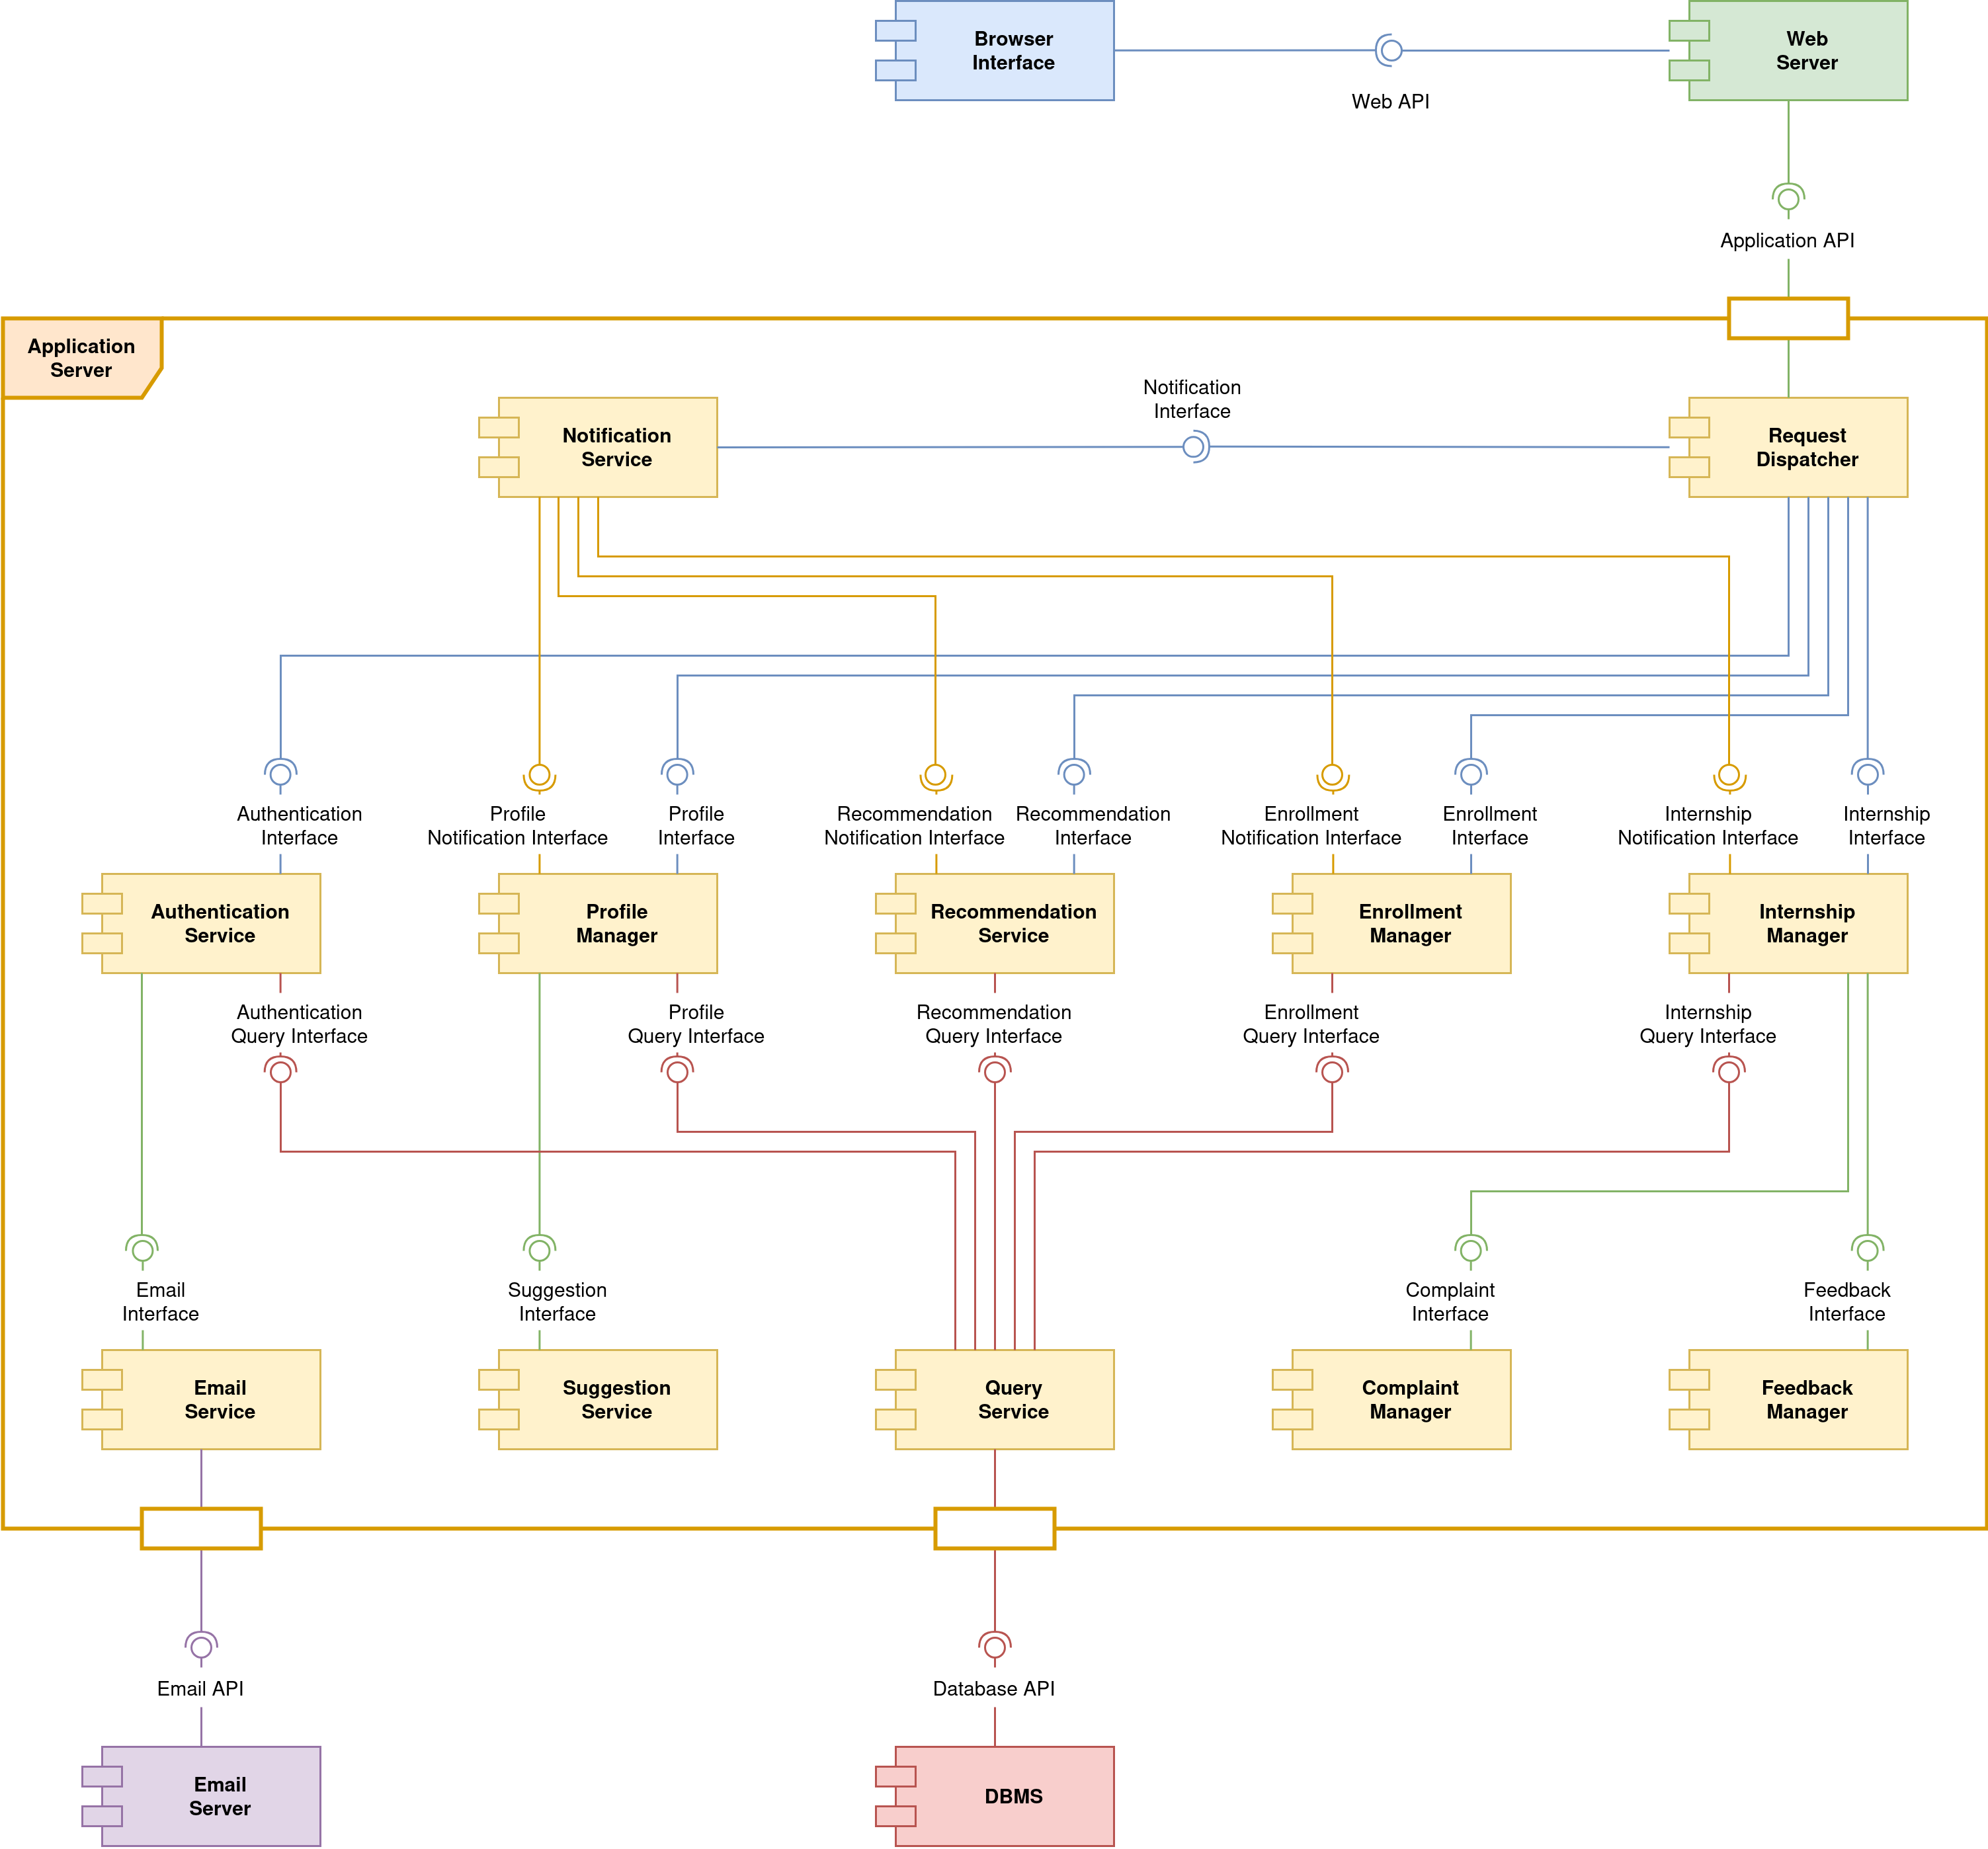
\includegraphics[width=0.8\linewidth]{../../assets/components-diagrams/components-diagram.png}
\end{figure}

\section{Deployment view}

The following diagram shows the deployment view of the system.
It illustrates the distribution of the components on the different nodes, and how they communicate between each others.

The system is composed of four tiers, one for the client frontend and three for the server fullstack processes: the client tier, the web tier, the application tier and the data tier.
The client tier corresponds to the web browser, which is required by the user to access the application.
The web tier represents the web server, which is used to handle incoming user requests and to return web pages and their content.
The application tier corresponds to the application server, that is used to execute the business logic and to communicate with the database.
The data tier is composed of the database, which is used to store all the data that the application server may require.

The email service is a set of external APIs used by the application to send emails to the users.

Moreover, since the platform will potentially need to manage a lot of concurrent users, the implementation of load balancers can help distribute the load among multiple servers.
This allows the application to be more scalable, since it eases the addition of other servers to handle an increasing load.
Those are placed between the client and the web server, and between the web server and the application server.

Lastly, to protect the application from external attacks, multiple firewalls are in use to filter the traffic.
In particular, those are placed between the client and the web server, between the web servers and the application server, and before the database.
This allows the application to execute in a more secure environment, since the firewall will filter the traffic before it reaches the designeted component.

\begin{figure}[H]
    \centering
    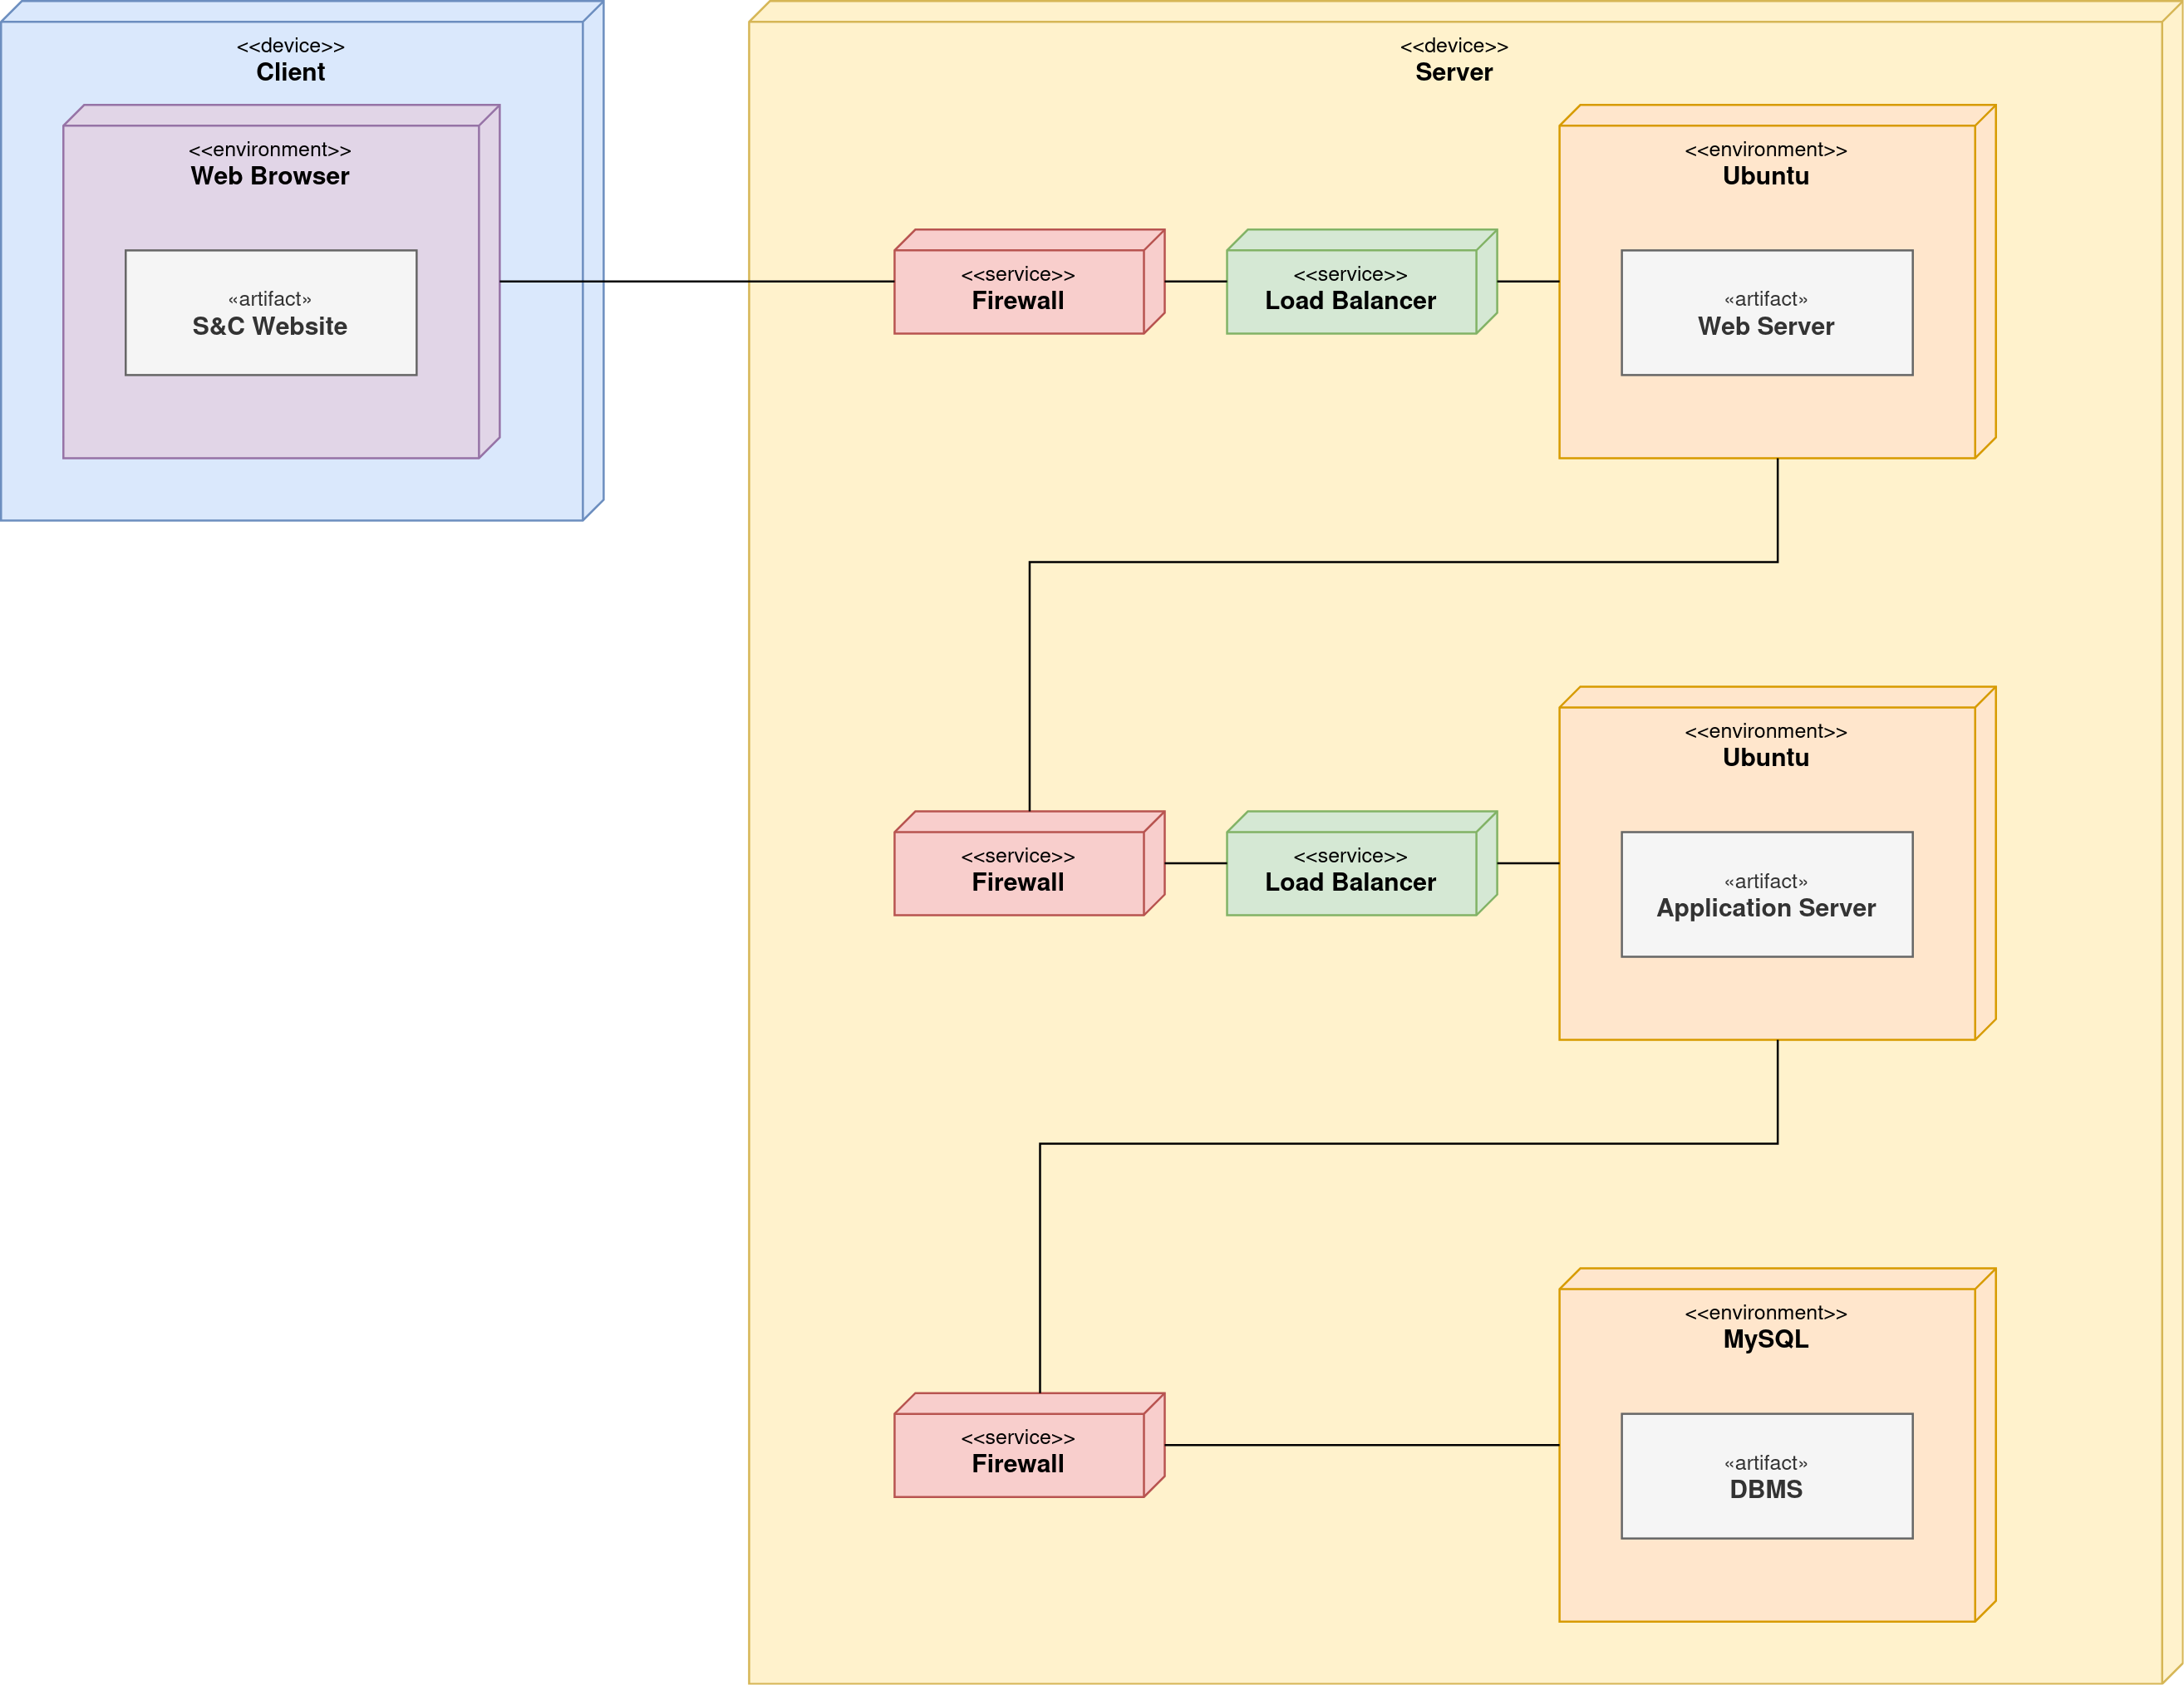
\includegraphics[width=0.8\linewidth]{../../assets/deployment-diagrams/deployment-diagram.png}
\end{figure}

\section{Runtime view}

This section contains the sequence diagrams of the most important operations of the system.
The diagrams include the component described in the previous sections, and the external components that are involved in the operations.

\begin{enumerate}[label=\textbf{RV\arabic* -}]

\item \subsubsection{StudentSignsUp}
\item \subsubsection{CompanySignsUp}
\item \subsubsection{UserLogsIn}
\item \subsubsection{StudentUploadsCV}
\item \subsubsection{CompanyCreatesAdvertisement}
\item \subsubsection{StudentVisualizesAdvertisements}
\item \subsubsection{CompanyVisualizesCandidates}
\item \subsubsection{CompanyCreatesQuestionnaire}
\item \subsubsection{StudentFillsQuestionnaire}
\item \subsubsection{CompanyAcceptsStudentEnrollment}
\item \subsubsection{StudentVisualizesInternshipInformation}
\item \subsubsection{CompanyVisualizesInternshipsInformation}
\item \subsubsection{StudentSendsComplaint}
\item \subsubsection{CompanySendsComplaint}
\item \subsubsection{UniversityVisualizesComplaints}
\item \subsubsection{UniversityEndsInternship}
\item \subsubsection{InternshipExpires}
\item \subsubsection{ParticipantFillsFeedbackForm}

\end{enumerate}

\section{Component interfaces}

\subsection{Application APIs}

\subsubsection{POST api/register}
\begin{itemize}
    \item Description: user is registered from form information
    \item Request body - \verb|{user: RegistrationForm}|
    \item Response 201 - Created
    \item Response 400 - Validation Error \verb|{error: Error}|
\end{itemize}

\subsubsection{POST api/register/verification/\{verificationID\}}
\begin{itemize}
    \item Description: user is verified through the verification code
    \item Response 201 - Created
    \item Response 400 - Validation Error \verb|{error: Error}|
\end{itemize}

\subsubsection{POST api/login}
\begin{itemize}
    \item Description: authentication token is returned if credentials are correct
    \item Request body - \verb|{user: Credentials}|
    \item Response 200 - OK \verb|{UserID: String, token: String}|
    \item Response 401 - Unauthorized \verb|{error: Error}|
\end{itemize}

\subsubsection{GET api/profile}
\begin{itemize}
    \item Description: user profile information is returned
    \item Request header - \verb|{Authorization: Bearer <token>}|
    \item Response 200 - OK \verb|{profile: ProfileData}|
    \item Response 400 - Invalid File \verb|{error: Error}|
    \item Response 401 - Unauthorized \verb|{error: Error}|
\end{itemize}

\subsubsection{POST api/profile}
\begin{itemize}
    \item Description: user profile information is updated
    \item Request header - \verb|{Authorization: Bearer <token>}|
    \item Request body - \verb|{profile: ProfileData}|
    \item Response 200 - OK
    \item Response 400 - Invalid File \verb|{error: Error}|
    \item Response 401 - Unauthorized \verb|{error: Error}|
\end{itemize}

\subsubsection{GET api/profile/cv}
\begin{itemize}
    \item Description: CV file is downloaded
    \item Request header - \verb|{Authorization: Bearer <token>}|
    \item Response 200 - OK \verb|{cv: File}|
    \item Response 400 - Invalid File \verb|{error: Error}|
    \item Response 401 - Unauthorized \verb|{error: Error}|
\end{itemize}

\subsubsection{POST api/profile/cv}
\begin{itemize}
    \item Description: CV file is uploaded
    \item Request header - \verb|{Authorization: Bearer <token>}|
    \item Request body - \verb|{cv: File}|
    \item Response 200 - OK
    \item Response 400 - Invalid File \verb|{error: Error}|
    \item Response 401 - Unauthorized \verb|{error: Error}|
\end{itemize}

\subsubsection{GET api/advertisements}
\begin{itemize}
    \item Description: a set of advertisements is returned
    \item Request header - \verb|{Authorization: Bearer <token>}|
    \item Response 200 - OK \verb|{advertisements: Advertisement[]}|
    \item Response 400 - Validation Error \verb|{error: Error}|
    \item Response 401 - Unauthorized \verb|{error: Error}|
\end{itemize}

\subsubsection{POST api/advertisements}
\begin{itemize}
    \item Description: an advertisement is created
    \item Request header - \verb|{Authorization: Bearer <token>}|
    \item Request body - \verb|{advertisement: Advertisement}|
    \item Response 201 - Created
    \item Response 400 - Validation Error \verb|{error: Error}|
    \item Response 401 - Unauthorized \verb|{error: Error}|
\end{itemize}

\subsubsection{GET api/candidates}
\begin{itemize}
    \item Description: a set of candidates is returned
    \item Request header - \verb|{Authorization: Bearer <token>}|
    \item Response 200 - OK \verb|{candidates: Candidate[]}|
    \item Response 400 - Validation Error \verb|{error: Error}|
    \item Response 401 - Unauthorized \verb|{error: Error}|
\end{itemize}

\subsubsection{GET api/applications}
\begin{itemize}
    \item Description: application requests are returned
    \item Request header - \verb|{Authorization: Bearer <token>}|
    \item Response 200 - OK \verb|{applications: Application[]}|
    \item Response 400 - Validation Error \verb|{error: Error}|
    \item Response 401 - Unauthorized \verb|{error: Error}|
\end{itemize}

\subsubsection{POST api/applications}
\begin{itemize}
    \item Description: the application request is registered
    \item Request header - \verb|{Authorization: Bearer <token>}|
    \item Request body - \verb|{application: Application}|
    \item Response 201 - Created
    \item Response 400 - Validation Error \verb|{error: Error}|
    \item Response 401 - Unauthorized \verb|{error: Error}|
\end{itemize}

\subsubsection{POST api/application/\{applicationID\}}
\begin{itemize}
    \item Description: the application request is accepted
    \item Request header - \verb|{Authorization: Bearer <token>}|
    \item Response 200 - OK
    \item Response 400 - Validation Error \verb|{error: Error}|
    \item Response 401 - Unauthorized \verb|{error: Error}|
\end{itemize}

\subsubsection{POST api/questionnaires}
\begin{itemize}
    \item Description: a custom questionnaire is created
    \item Request header - \verb|{Authorization: Bearer <token>}|
    \item Request body - \verb|{questionnaire: Questionnaire}|
    \item Response 201 - Created
    \item Response 400 - Validation Error \verb|{error: Error}|
    \item Response 401 - Unauthorized \verb|{error: Error}|
\end{itemize}

\subsubsection{GET api/questionnaires/\{questionnaireID\}}
\begin{itemize}
    \item Description: the questionnaire is returned
    \item Request header - \verb|{Authorization: Bearer <token>}|
    \item Response 200 - OK \verb|{questionnaire: Questionnaire}|
    \item Response 400 - Validation Error \verb|{error: Error}|
    \item Response 401 - Unauthorized \verb|{error: Error}|
\end{itemize}

\subsubsection{POST api/questionnaires/\{questionnaireID\}}
\begin{itemize}
    \item Description: the filled in questionnaire is stored
    \item Request header - \verb|{Authorization: Bearer <token>}|
    \item Request body - \verb|{questionnaire: Questionnaire}|
    \item Response 201 - Created
    \item Response 400 - Validation Error \verb|{error: Error}|
    \item Response 401 - Unauthorized \verb|{error: Error}|
\end{itemize}

\subsubsection{GET api/proposals}
\begin{itemize}
    \item Description: proposals are returned
    \item Request header - \verb|{Authorization: Bearer <token>}|
    \item Response 200 - OK \verb|{proposals: Proposal[]}|
    \item Response 400 - Validation Error \verb|{error: Error}|
    \item Response 401 - Unauthorized \verb|{error: Error}|
\end{itemize}

\subsubsection{POST api/proposals}
\begin{itemize}
    \item Description: a proposal is registered
    \item Request header - \verb|{Authorization: Bearer <token>}|
    \item Request body - \verb|{proposal: Proposal}|
    \item Response 201 - Created
    \item Response 400 - Validation Error \verb|{error: Error}|
    \item Response 401 - Unauthorized \verb|{error: Error}|
\end{itemize}

\subsubsection{POST api/proposals/\{proposalID\}}
\begin{itemize}
    \item Description: the proposal is accepted
    \item Request header - \verb|{Authorization: Bearer <token>}|
    \item Response 200 - OK
    \item Response 400 - Validation Error \verb|{error: Error}|
    \item Response 401 - Unauthorized \verb|{error: Error}|
\end{itemize}

\subsubsection{GET api/internships}
\begin{itemize}
    \item Description: internship information is returned
    \item Request header - \verb|{Authorization: Bearer <token>}|
    \item Response 200 - OK \verb|{internship: Internship}|
    \item Response 400 - Validation Error \verb|{error: Error}|
    \item Response 401 - Unauthorized \verb|{error: Error}|
\end{itemize}

\subsubsection{GET api/internship/\{internshipID\}/complaints}
\begin{itemize}
    \item Description: complaints about an internship are returned
    \item Request header - \verb|{Authorization: Bearer <token>}|
    \item Response 200 - OK \verb|{complaints: Complaint[]}|
    \item Response 400 - Validation Error \verb|{error: Error}|
    \item Response 401 - Unauthorized \verb|{error: Error}|
\end{itemize}

\subsubsection{POST api/internship/\{internshipID\}/complaints}
\begin{itemize}
    \item Description: a complaint about an internship is created
    \item Request header - \verb|{Authorization: Bearer <token>}|
    \item Request body - \verb|{complaint: Complaint}|
    \item Response 201 - Created
    \item Response 400 - Validation Error \verb|{error: Error}|
    \item Response 401 - Unauthorized \verb|{error: Error}|
\end{itemize}

\subsubsection{POST api/internship/\{internshipID\}/interrupt}
\begin{itemize}
    \item Description: the internship is interrupted
    \item Request header - \verb|{Authorization: Bearer <token>}|
    \item Response 200 - OK
    \item Response 400 - Validation Error \verb|{error: Error}|
    \item Response 401 - Unauthorized \verb|{error: Error}|
\end{itemize}

\subsubsection{POST api/internships/\{internshipID\}/feedback}
\begin{itemize}
    \item Description: a filled in feedback form about an internship is stored
    \item Request header - \verb|{Authorization: Bearer <token>}|
    \item Request body - \verb|{feedbackForm: FeedbackForm}|
    \item Response 201 - Created
    \item Response 400 - Validation Error \verb|{error: Error}|
    \item Response 401 - Unauthorized \verb|{error: Error}|
\end{itemize}

\subsubsection{GET api/notifications}
\begin{itemize}
    \item Description: the notifications of the user are returned
    \item Request header - \verb|{Authorization: Bearer <token>}|
    \item Response 200 - OK \verb|{notifications: Notification[]}|
    \item Response 400 - Validation Error \verb|{error: Error}|
    \item Response 401 - Unauthorized \verb|{error: Error}|
\end{itemize}

\subsection{Interface methods}

\subsubsection{Notification interface}
\begin{itemize}
    \item \verb|List<Notification> getNotificationList(user: User)|
\end{itemize}

\subsubsection{Profile notification interface}
\begin{itemize}
    \item \verb|boolean notify(user: User, notification: Notification)|
\end{itemize}

\subsubsection{Recommendation notification interface}
\begin{itemize}
    \item \verb|boolean notify(user: User, notification: Notification)|
\end{itemize}

\subsubsection{Enrollment notification interface}
\begin{itemize}
    \item \verb|boolean notify(user: User, notification: Notification)|
\end{itemize}

\subsubsection{Internship notification interface}
\begin{itemize}
    \item \verb|boolean notify(user: User, notification: Notification)|
\end{itemize}

\subsubsection{Authentication interface}
\begin{itemize}
    \item \verb|boolean registerUser(credentials: Credentials)|
    \item \verb|boolean verifyUser(verificationCode: String)|
    \item \verb|Token login(credentials: Credentials)|
    \item \verb|boolean logout(token: Token)|
    \item \verb|boolean validateToken(token: Token)|
\end{itemize}

\subsubsection{Profile interface}
\begin{itemize}
    \item \verb|User getUser(userID: String)|
    \item \verb|boolean updateProfile(user: User, updates: Map<String, String>)|
\end{itemize}

\subsubsection{Recommendation interface}
\begin{itemize}
    \item \verb|List<Advertisement> recommendedAdvertisements(student: Student)|
    \item \verb|List<Student> recommendedCandidates(company: Company, | \\ \makebox[10em][l]{} \verb|advertisement: Advertisement)|
    \item \verb|List<Advertisement> searchAdvertisements(searched: String)|
    \item \verb|List<Student> searchCandidates(searched: String)|
\end{itemize}

\subsubsection{Enrollment interface}
\begin{itemize}
    \item \verb|EnrollmentStatus getEnrollmentStatus(user: User, | \\ \makebox[10em][l]{} \verb|advertisement: Advertisement)|
    \item \verb|boolean requestApplication(student: Student, | \\ \makebox[10em][l]{} \verb|advertisement: Advertisement)|
    \item \verb|boolean buildQuestionnaire(company: Company, | \\ \makebox[10em][l]{} \verb|questionnaire: Questionnaire)|
    \item \verb|List<Questionnaire> getQuestionnaires(company: Company)|
    \item \verb|boolean sendQuestionnaire(company: Company, student: Student, | \\ \makebox[10em][l]{} \verb|questionnaire: Questionnaire)|
    \item \verb|boolean fillQuestionnaire(student: Student, | \\ \makebox[10em][l]{} \verb|questionnaire: Questionnaire)|
    \item \verb|boolean acceptEnrollment(company: Company, student: Student, | \\ \makebox[10em][l]{} \verb|Advertisement: advertisement)|
    \item \verb|boolean acceptProposal(student: Student, company: Company, | \\ \makebox[10em][l]{} \verb|Advertisement: advertisement)|
\end{itemize}

\subsubsection{Internship interface}
\begin{itemize}
    \item \verb|Internship getOngoingInternship(student: Student)|
    \item \verb|List<Internship> getOngoingInternships(company: Company)|
    \item \verb|boolean registerComplaint(user: User, internship: Internship, | \\ \makebox[10em][l]{} \verb|complaint: Complaint)|
    \item \verb|List<Complaint> getComplaints(university: University)|
    \item \verb|boolean interruptInternship(university: University, | \\ \makebox[10em][l]{} \verb|internship: Internship)|
    \item \verb|boolean registerFeedback(user: User, feedback: Feedback)|
\end{itemize}

\subsubsection{Email interface}
\begin{itemize}
    \item \verb|boolean sendEmail(email: Email, content: String)|
\end{itemize}

\subsubsection{Suggestion interface}
\begin{itemize}
    \item \verb|List<Suggestion> proposeProfileSuggestions(student: Student)|
    \item \verb|List<Suggestion> proposeAdvertisementSuggestions(| \\ \makebox[10em][l]{} \verb|Advertisement: advertisement)|
\end{itemize}

\subsubsection{Complaint interface}
\begin{itemize}
    \item \verb|boolean sendComplain(user: User, internship: Internship, | \\ \makebox[10em][l]{} \verb|complaint: Complaint)|
    \item \verb|List<Complaint> getComplaints(university: University)|
\end{itemize}

\subsubsection{Feedback interface}
\begin{itemize}
    \item \verb|boolean sendFeedback(user: User, feedback: Feedback)|
\end{itemize}

\subsubsection{Authentication query interface}
\begin{itemize}
    \item \verb|User getUser(credentials: Credentials)|
    \item \verb|boolean registerUser(credentials: Credentials)|
    \item \verb|boolean verifyUser(verificationCode: String)|
    \item \verb|boolean checkCredentials(credentials: Credentials)|
    \item \verb|boolean setToken(userID: String, token: Token)|
    \item \verb|boolean checkToken(userID: String, token: Token)|
    \item \verb|boolean deleteToken(userID: String)|
\end{itemize}

\subsubsection{Profile query interface}
\begin{itemize}
    \item \verb|User getUser(userID: String)|
    \item \verb|boolean updateProfile(userID: String, updates: Map<String, String>)|
\end{itemize}

\subsubsection{Recommendation query interface}
\begin{itemize}
    \item \verb|User getUser(userID: String)|
    \item \verb|List<Advertisement> getMatchingAdvertisements(keyWords: List<String>)|
    \item \verb|List<Student> getMatchingCandidates(keyWords: List<String>)|
\end{itemize}

\subsubsection{Enrollment query interface}
\begin{itemize}
    \item \verb|User getUser(userID: String)|
    \item \verb|EnrollmentStatus getEnrollmentStatus(userID: String, | \\ \makebox[10em][l]{} \verb|advertisementID: String)|
    \item \verb|boolean requestApplication(userID: String, advertisementID: String)|
    \item \verb|boolean buildQuestionnaire(userID: String, questionnaire: Questionnaire)|
    \item \verb|List<Questionnaire> getQuestionnaires(userID: String)|
    \item \verb|boolean sendQuestionnaire(companyID: String, studentID: String, | \\ \makebox[10em][l]{} \verb|questionnaireID: String)|
    \item \verb|boolean fillEnrollment(studentID: String, questionnaire: Questionnaire)|
    \item \verb|boolean sendQuestionnaire(companyID: String, studentID: String, | \\ \makebox[10em][l]{} \verb|questionnaireID: String)|
    \item \verb|boolean acceptProposal(studentID: String, companyID: String, | \\ \makebox[10em][l]{} \verb|advertisementID: String)|
\end{itemize}

\subsubsection{Internship query interface}
\begin{itemize}
    \item \verb|User getUser(userID: String)|
    \item \verb|Internship getOngoingInternship(userID: String)|
    \item \verb|List<Internship> getOngoingInternships(userID: String)|
    \item \verb|boolean registerComplaint(userID: String, internshipID: String, | \\ \makebox[10em][l]{} \verb|complaint: Complaint)|
    \item \verb|List<Complaint> getComplaints(userID: String)|
    \item \verb|boolean interruptInternship(internshipID: String)|
    \item \verb|boolean registerFeedback(userId: User, feedback: Feedback)|
\end{itemize}

\section{Architectural styles and patterns}

\htitle{Three-tier architecture}
Since the S\&C platform is offered through the web, the client-server architecture is the most suitable for this kind of application.
In particular, a three-tier architecture comes handy when dividing the system into the three main logical layers: presentation (web server), business logic (application server), and data storage (database).
Each tier has its specific functions, ensuring separation of concerns and efficient management of the system.
It allows scalability, simplifies maintenance, and enhances control and security.

\htitle{REST}
The communication between the web server and the application server is based on the REST architectural style.
REST is stateless, meaning that the server does not need to store any information about the session, allowing higher scalability.
Moreover, it provides a uniform and easy interface via the HTTP methods (GET, POST, PUT, DELETE).

\htitle{MVC}
The MVC pattern is used to separate the presentation layer from the business logic.
In particular, the model contains the definitions of all the elements of the application, the view is the browser interface component, and the controller comprehends all the other application server services and managers.
This pattern allows a more maintainable application, since changes in one layer do not affect other layers.

\section{Other design decisions}

\htitle{Scale out}
Using a scale out design, when implementing the software, can highly enhance availability, by avoiding the need of downtimes.
This design approach enables the system to expand its capacity to cope with an increasing demand, by adding more resources when needed.
Moreover, it can be more cost effective than upgrading individual components.
The scale out design also improves reliability, by providing redundant resources that can take over when other components fails.
Flexibility is also augmented, as resources can be fastly added or removed, as required.
Lastly, the scale out design improves the system performance, since workloads are processed in parallel rather than sequentially.

\htitle{Relational database}
Due to its effectiveness at storing structured data, a relational database was chosen for the system design.
It also enforces data integrity while providing fast query performance.
A relational DB is also able to handle large amounts of data, while supporting many concurrent users.

\htitle{Token-based authentication}
The authentication and authorization is implemented using a token-based process.
These tokens are sent to the users each time they log in, and they must be included within each request that requires authentication or authorization.

